\documentclass[a4paper, twocolumn]{article}
\usepackage[utf8]{inputenc}
\usepackage[french]{babel}
\usepackage{graphicx}

\begin{document}

	\title{Rapport de Mini-Projet 3I025 \\
		\large Recherche de chemins coopératifs entre agents}
	\author{Castellon Clément \and Zhang Noé}
	\maketitle

	\part{Introduction}
	
		Durant les dernières années, plusieurs nouvelles technologies ont commencé à faire leur émergence, parmi elles nous pouvons retrouver les techniques autonomes qui apparaissent de plus en plus dans notre vie quotidienne. En effet nous retrouvons notemment la célèbre application de commande vocale Siri mais aussi d'autres tels que les voitures autonomes ceux-ci pouvant être considérés comme des agents autonomes.
		Il convient alors d'étudier comment ces agents sont capables de subsister sans intervention humaine. 
		
		\section{Projet}
		
		\subsection{Sujet}
		Nous considérons plusieurs agents en compétition qui cherchent chacun à atteindre leur propre objectif sans qu'il y ait des collisions entre les différents agents.
		Nous cherchons à maximiser la coopération entre les agents autrement dit, minimiser le temps total nécessaire à ce que chacun d'eux atteignent son objectif.
		
		\subsection{Approches}
		Trois solutions différentes sont proposées afin de répondre au problème de collision. La première solution consiste à utiliser une stratégie de path-splicing. La seconde tend à ordonner les trajets exécutés dans un ordre sans collision. Enfin la troisième utilise une table de réservation de coordonnées dans le temps.
	
		\section{Notions de base}
		
		\subsection{Agents Intelligents}
		Un agent intelligent peut-être considéré comme une entité autonome capable d'exécuter des services ou de prendre des décisions en fonction de son environnement et cela sans intervention humaine. Afin de pouvoir remplir ses objectifs, un agent doit posséder plusieurs caractéristiques. Tout d'abord, il doit être capable d'interagir avec son environnement et de s'adapter en conséquence. Dans un contexte plus avancé, il doit savoir profiter de ses expériences passées afin de mieux comprendre les souhaits de l'utilisateur et, lors du déploiement de plusieurs agents, doit pouvoir communiquer et interagir avec eux afin de maximiser la coopération et ainsi les performances globales. En faisant varier ses caractéristiques, il est alors possible de créer différents types d'agents qui répondent au mieux aux exigences de l'utilisateur.
		
		\subsection{Collisions}
		Lors du déplacement des agents, deux types de collisions différentes peuvent apparaître entre les agents. En effet, la première occure lorsque deux agents différents veulent accéder à la même case à un instant 't' identique a contrario, la seconde apparaît lorsque deux agents sont face à face et veulent tous deux accéder à leur position courante respective.
		
	\setcounter{section}{0}
	\part{Stratégies}

		\section{Path-Splicing}

			\subsection{Idée globale}
			Dans cette première implémentation, l'idée consiste à modifier le chemin emprunté par un agent seulement lorsque celui-ci détecte une collision c'est-à-dire à l'instant précédant la collision, en effet lorsqu'un agent détecte une collision avec un autre, il va considérer le lieu de collision comme un obstacle et va calculer en conséquence un nouveau chemin qui lui permettra d'atteindre un état postérieur de son chemin en tenant compte du lieu de collision.

			\subsection{Implémentation}
			Dans un premier temps chaque agent calcule indépendamment des autres des chemins lui permettant d'atteindre son objectif, pour cela nous avons utilisé l'algorithme A* qui permet de calculer le plus court chemin entre deux coordonnées.
			Une fois les chemins calculés, nous les gardons en mémoire et associons à chaque agent un compteur qui correspond à l'étape où se trouve celui-ci dans son chemin associé.
			Lorsqu'une collision est détectée deux comportements peuvent apparaître.
			En effet, le premier cas se produit lorsque le lieu de collision de l'agent a lieu sur la position de son objectif, et le second lorsque la collision a lieu sur une case autre que l'objectif.
			Dans le premier cas, l'agent qui détecte la collision va effectuer un pas aléatoire puis recalculer un chemin jusqu'à son objectif. Tandis que dans le second cas, l'agent va calculer un chemin alternatif qui l'amènera à la position deux étapes plus tard dans son chemin tout en considérant le lieu de collision comme un obstacle. Les coordonnées de la collision sont alors remplacées par le nouveau chemin.
			
			\subparagraph{}
			Dans le cas général cette implémentation fournit de bons résultats cependant, il peut y avoir des cas où l'algorithme des chemins bien plus longs que nécessaires réduisant ainsi les performances.

		\section{Coopération de base}

			\subsection{Idée globale}
			Dans cette seconde stratégie, les agents se déplacent par groupes. Les groupes sont formés tels qu aucun chemin appartenant au même groupe n'est en collision avec un autre chemin du même groupe. Différentes stratégies peuvent être implémentées afin de définir l'ordre de passage et ainsi modifier les paramètres maximisés.

			\subsection{Implémentation}
			Tout d'abord, chaque agent calcule un chemin vers son objectif en tenant compte de la position courante des autres agents, ce traitement est effectué avec l'algorithme A étoile. Par la suite, des groupes sont formés tel que les chemins des agents d'un même groupe ne forment pas de collisions s'ils sont exécutés en même temps. 
			L'ordre de passage des groupes est alors organisé grâce à une stratégie définie par l'utilisateur. Comme stratégie de base, nous utilisons une stratégie FIFO revisitée qui consiste dans un premier temps à prendre le premier groupe formé et à l'exécuter. Ensuite, lorsque tout les agents de ce groupe ont terminé d'exécuter leur chemin, leur chemin est recalculé et ils sont ensuite insérés dans le nouveau groupe. Afin d'éviter la famine, les agents sont ajoutés en partant de la fin de la file.
			Enfin, avant d'envoyer le prochain groupe on va recalculer leur chemin en tenant compte de la nouvelle position courante des agents du groupe terminé. Si deux nouveaux chemins formés produisent une collision on en enlève un des deux et on exécute le groupe.

			\subparagraph{}
			Cette implémentation se rapproche de l'implémentation naïve qui consiste à exécuter chaque chemin lorsque le précédent est terminé. La coopération n'est que très peu optimisée, cependant son implémentation est plus simple que les autres.

		\section{Coopération avancée}

			\subsection{Idée globale}
			Dans cette dernière implémentation, nous utilisons une structure de données partagée par tous les agents qui contient les cases des chemins de chaque agent à l'instant réservé 't'. Un emplacement est considéré comme collision seulement si la position de celui-ci est déjà réservée par un autre joueur au même instant où à l'instant suivant. 
			Contrairement aux stratégies précédentes, nous calculons ici des chemins partiels vers l'objectif, l'heuristique utilisée est alors la vrai distance entre la position du joueur et celle de son objectif, autrement dit, il s'agit de la taille du chemin minimum qui sépare les deux positions. 

			\subsection{Implémentation}
			
			\subsubsection{Table de réservation}
			Les chemins des agents sont créés séquentiellement tout en tenant compte du chemin des agents précédents. En effet lors de la création de son chemin, chaque agent va regarder dans la table de réservation si la case choisie n'a pas déjà été réservée au même instant par un autre joueur, si tel est le cas, la case est alors considérée comme un obstacle, sinon la case sera réservée par ce joueur à l'instant où il y passe. Pour cela des doublets 'coordonnées, time' sont stockés dans un dictionnaire comme les clés de celui-ci auxquels on associe le joueur qui a réservé la position.
		
			
			\subsubsection{A* Espace-Temps}
			L'heuristique utilisé dans cette implémentation est la vraie distance entre la position du joueur et celle de son objectif. Afin de retrouver cette valeur rapidement, on effectue une recherche de chemin en prenant l'objectif de l'agent comme point de départ de l'algorithme A* jusqu'à la position courante. La vraie distance correspond alors à la valeur g de la position du joueur par rapport à cette deuxième recherche. Afin d'améliorer les performances, cette recherche n'est effectuée qu'une seule fois par chemin par agent mais peut-être relancée à partir de l'état précédent si besoin.

			\subsubsection{Chemin partiel}
			Nous limitons la longueur des chemins de chaque agent. En effet, le fait de limiter la longueur du chemin permet à l'agent de récupérer de nouvelles informations sur son environnement évitant une trop grande perte de travail de la part de celui-ci si des modifications ont eu lieu.
			Le chemin partiel n'affecte pas la direction de l'agent puisqu'il s'agit de la vrai distance qui est utilisée comme heuristique.

			\subparagraph{}
			Cette solution plus complexe que les précédentes offrent une solution plus avancée au problème des collisions notemment grâce à l'ajout de la troisième dimension, le temps, qui permet aux agents d'obtenir plus d'informations sur leur environnement.

		\section{Observation}
		
		Les implémentations proposées possèdent chacune des avantages et des inconvénients que nous allons étudier dans la partie suivante.
		
		\subsection{Performance des implémentations}
		
		\begin{figure}[h!]
			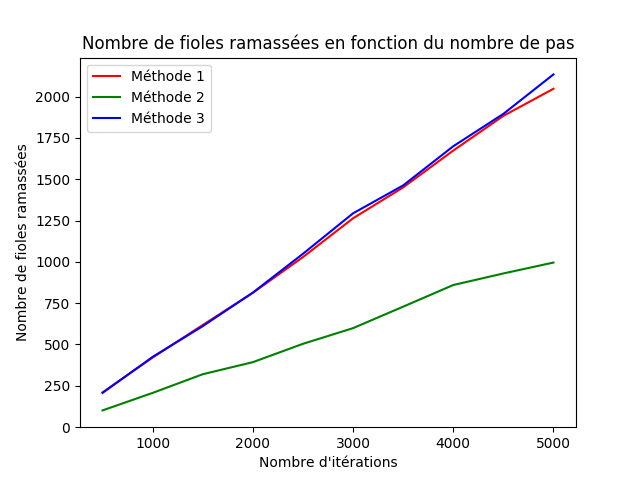
\includegraphics[width=3.2in]{compare_methods.png}
			\caption{\textsf{Perfomances des différentes méthodes en fonction du nombre de pas}}
			\label{fig_sim}
		\end{figure}
	
		Les performances sont observées par rapport au nombre totale de fioles ramassées par tout les agents en fonction du nombre d'itérations. Dans un premier temps, nous pouvons observer que les performances de la méthode d'ordonnancement par groupe sont représentées par une droite avec une faible pente tandis que celles des deux autres méthodes semblent être chacunes représentées par une droite avec une pente plus élevée. De plus, parmis les deux méthodes possédant des performances linéaires, nous pouvons observer que leurs résultats sont très proches, cependant la troisième méthode prend légèrement le dessus sur la première méthode après un seuil de trois mille pas.
		
		Aux vues de nos observations la méthode de path-splicing et la méthode utilisant une table de réservation semblent être un meilleur choix puisque les performances de ces deux implémentations sont très largement supérieures à la méthode utilisant un ordonnancement par groupe. On observe que les performances de la première méthode sont proches de celles de la troisième, cela peut-être expliqué grâce à la carte utilisée. En effet nos cartes sont de petite taille avec peu d'agents, favorisant ainsi la première méthode qui ne recalcule que peu souvent un nouveau chemin alternatif, et souvent la taille de ce chemin reste très court.
		
		\subsection{Temps CPU}
		
		\begin{figure}[h!]
			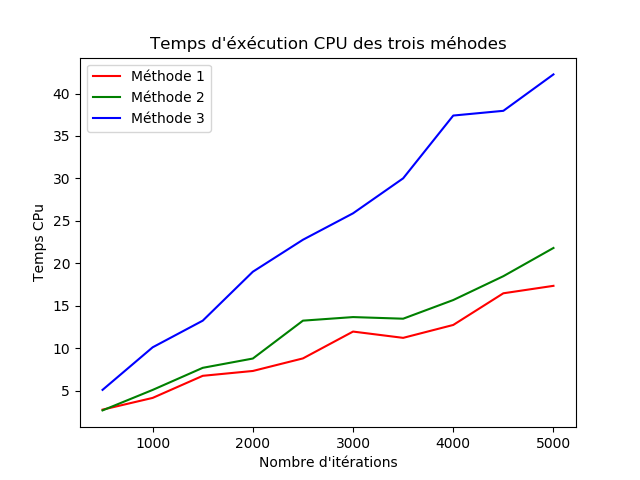
\includegraphics[width=3.2in]{CPU_time.png}
			\caption{\textsf{Performances des différentes méthodes en fonction du nombre de pas}}
			\label{fig_sim}
		\end{figure}
	
		Le temps d'exécution CPU correspond au temps nécessaire pour exécuter un certain nombre d'itérations. Ainsi, nous observons que la troisième méthode se distingue très largement des deux premières, en effet le temps nécessaire à l'exécution des itérations est près de deux fois supérieur au temps nécessaires pour les deux autres méthodes. Aussi, parmis ces deux autres méthodes, nous pouvons observer un temps légèrement plus élevé pour la deuxième méthode.
		
		Le temps d'exécution élevé de la part de la troisième méthode semble provenir du calcul de l'heurisique qui nécessite d'utiliser l'algorithme A étoile plus souvent sur de longs chemins.
		Pour les deux autres méthodes les temps d'exécution sont proches, puisque l'algortihme A étoile est calculé un nombre fixe de fois pour la deuxième méthode et, plusieurs fois mais sur des chemins de courte taille pour la première.
	 
	 	En prenant en compte les deux facteurs que sont le temps d'exécution et le nombre total de fioles ramassées une implémentation semble sortir du lot. En effet de part sa simplicité et des résultats qu'elle nous apporte la méthode utilisant le path-splicing semble être la meilleure alternative à notre problème de collisions.
		
	\part{Conclusion}
	Au cours de ce projet, nous avons pu expérimenter différentes stratégies, chacune possédant leurs points forts et leurs points faibles. Au vu des résultats obtenus, le choix de la stratégie optimal semble dépendre de l'environnement dans lequel celle-ci va être utilisée. Pour des environnement triviaux où le nombre d'agents est faible, il semble préférable d'utiliser une méthode qui possède une implémentation simple et un bon temps CPU tandis que pour un environnement complexe il conviendra de se diriger vers une méthode plus recherchée permettant de meilleures performances.

\end{document}
